\documentclass[11pt,a4paper]{article}

\usepackage[utf8]{inputenc}
\usepackage[margin=2.5cm]{geometry}
\usepackage{amsmath,amssymb,amsthm,mathtools}
\usepackage{booktabs,array}
\usepackage{enumitem}
\usepackage{tikz}
\usepackage[colorlinks=true,linkcolor=blue!50!black,citecolor=blue!50!black,urlcolor=blue!50!black]{hyperref}

% ---------- macros ----------
\newcommand{\ii}{\mathrm{i}}
\newcommand{\dd}{\mathrm{d}}
\newcommand{\eps}{\varepsilon}
\newcommand{\R}{\mathbb{R}}
\newcommand{\bx}{\mathbf{x}}
\newcommand{\bv}{\mathbf{v}}
\newcommand{\bp}{\mathbf{p}}
\newcommand{\bu}{\mathbf{u}}
\newcommand{\bE}{\mathbf{E}}
\newcommand{\bB}{\mathbf{B}}
\newcommand{\bA}{\mathbf{A}}
\newcommand{\bJ}{\mathbf{J}}
\newcommand{\bP}{\mathbf{P}}
\newcommand{\gal}{\mathfrak{gal}}
\newcommand{\poinc}{\mathfrak{iso}(3,1)}
\emergencystretch=3em

\theoremstyle{plain}
\newtheorem{proposition}{Proposition}
\theoremstyle{definition}
\newtheorem{definition}{Definition}
\theoremstyle{remark}
\newtheorem{remark}{Remark}

\title{Newtonian Mechanics Is Not a Limit of Relativistic Mechanics:\\[2pt]
Algebraic and Geometric Structure, and Why a Charged Particle\\
in an Electromagnetic Field Is Different}
\author{}   % <-- add author name(s) here
\date{\today}

\begin{document}
\maketitle

\begin{abstract}
\noindent
It is often said that Newtonian mechanics is the limit $c\to\infty$ of special-relativistic
mechanics. We argue that this is true for \emph{formulas} and for \emph{solutions of particular
systems in particular regimes}, but false for \emph{structures}. The Galilei group is not a
member of a continuous family of mutually isomorphic groups containing the Poincar\'e group: it
is a \emph{singular contraction} of it, with a different Levi decomposition, a non-trivial central
extension (the mass), and no counterpart of the four-vector structure of energy--momentum.
Geometrically, the non-degenerate Lorentzian metric is replaced by a pair of degenerate
structures (absolute time and a spatial metric) which do not determine the connection;
the light cones collapse onto hyperplanes of simultaneity. Dynamically, interaction among
particles through instantaneous potentials is compatible with Galilean invariance but,
by the no-interaction theorem, not with Poincar\'e invariance of a Hamiltonian particle theory.
Against this background we show that a charged particle in a \emph{prescribed} electromagnetic
field does possess a non-relativistic limit, classically (Lorentz force from the expanded
Lagrangian) and quantum mechanically (Dirac $\to$ Pauli). We identify the structural reasons:
the mass-shell hyperboloid flattens, the divergent rest energy is a removable central term,
and the magnetic field of the external source survives only in a double limit $c\to\infty$,
$N\to\infty$ (macroscopic currents or magnetisation, $N\sim c^2$), whose scaling is transparent in
Gaussian units and hidden in SI; with that scaling the field transforms under Galilei boosts.
Electromagnetism itself has two inequivalent Galilean limits, and neither contains radiation.
\end{abstract}

%=====================================================================
\section{Introduction}
%=====================================================================
It is a commonplace that Newtonian mechanics is ``the limit $c\to\infty$'' of special
relativity. The usual evidence is a pair of expansions,
\begin{equation}\label{eq:expansions}
\gamma=\Bigl(1-\frac{v^2}{c^2}\Bigr)^{-1/2}=1+\frac{v^2}{2c^2}+O(c^{-4}),
\qquad
E=\sqrt{p^2c^2+m^2c^4}=mc^2+\frac{p^2}{2m}+O(c^{-2}).
\end{equation}
The sentence hides two logically different claims.
\begin{description}[leftmargin=1.2cm,style=nextline]
\item[(A) Asymptotic reading.] For a given physical system and given data with $|\bv|\ll c$,
the relativistic solutions differ from the Newtonian ones by terms of relative size
$O(v^2/c^2)$.
\item[(B) Structural reading.] A theory is a package: a symmetry group, a spacetime geometry,
an algebra of observables with its Poisson (or commutator) structure, a space of states,
and rules for coupling. The relativistic package depends on the parameter
$\kappa:=c^{-2}$, and the Newtonian package is the member $\kappa=0$ of the \emph{same}
continuous family.
\end{description}
Reading (A) is a statement about numbers; reading (B) is a statement about structures.
They are logically independent. We shall argue that (B) fails in a precise sense, that (A) fails for
some natural systems (several interacting particles) while holding for others, and that a charged
particle in a prescribed electromagnetic field is one of the systems for which it holds, for
reasons that can be stated in structural terms.

Nothing here says that Newtonian mechanics is ``wrong'' or that its predictions cannot be derived
from relativistic ones for slow motion. The point is about the \emph{kind} of relation between the
two theories: it is a degeneration (contraction) rather than a regular limit. This viewpoint goes
back to work on contractions of groups \cite{Segal51,IW53,Saletan61}, to the classification of
kinematical groups \cite{BLL68}, and to the philosophical literature on singular limits and
reduction \cite{Nickles73,Berry94,Batterman02}; the opposite direction---relativity as a
\emph{deformation} of Newtonian kinematics---is emphasised in \cite{Dyson72,VM94}.

The plan is as follows. Section~\ref{sec:limits} fixes what ``limit'' can mean.
Section~\ref{sec:algebra} compares the Poincar\'e and Galilei algebras and their representations,
Section~\ref{sec:geometry} the corresponding geometries, and Section~\ref{sec:dynamics} the
dynamics of interacting particles. Section~\ref{sec:EM} treats the charged particle in an
electromagnetic field, and Section~\ref{sec:conclusion} concludes.

\emph{Conventions.} The Minkowski metric has signature $(+,-,-,-)$. Electromagnetic formulae are
written in Gaussian units; Section~\ref{ssec:units} explains why this matters for the limit.

%=====================================================================
\section{What can ``limit'' mean?}\label{sec:limits}
%=====================================================================
Let $\kappa=c^{-2}\ge 0$ and let $\mathcal S_\kappa$ denote a structure (a Lie algebra, a
manifold with tensor fields, a Poisson algebra) depending on $\kappa$ in some fixed set of
coordinates. For Lie algebras the following terminology is standard.

\begin{definition}[Contraction]
Let $(V,[\cdot,\cdot])$ be a Lie algebra and $U_\kappa\in GL(V)$ a family of linear maps. Put
$[x,y]_\kappa:=U_\kappa^{-1}[U_\kappa x,U_\kappa y]$. If $[x,y]_\kappa\to[x,y]_0$ for $\kappa\to 0$
and $[\cdot,\cdot]_0$ is a Lie bracket \emph{not} isomorphic to $[\cdot,\cdot]$, then
$(V,[\cdot,\cdot]_0)$ is a \emph{contraction} of $(V,[\cdot,\cdot])$, and the limit is called \emph{singular}.
\end{definition}

Every $[\cdot,\cdot]_\kappa$ with $\kappa>0$ is isomorphic to the original algebra by construction;
the change of basis $U_\kappa$ is what diverges (or degenerates) as $\kappa\to 0$. In the space of
structure constants, the orbit of $[\cdot,\cdot]_0$ lies in the closure of the orbit of
$[\cdot,\cdot]$ but has strictly smaller dimension: the limit object has a \emph{larger}
automorphism group than the generic member. A limit in this sense therefore changes the
isomorphism type. Quantities that are defined by the isomorphism type of the generic member (its
Levi factor, its invariant forms, its cohomology) need not have limits at all.

At the level of dynamics the analogue is Berry's notion of a singular limit
\cite{Berry94,Batterman02}: the limit of the solutions is not the solution of the limiting
equation, or the limiting equation is of a different type (order, character) than the members of
the family. Both phenomena occur in the passage from relativistic to Newtonian mechanics, as we
shall see.

%=====================================================================
\section{Algebraic structure}\label{sec:algebra}
%=====================================================================

\subsection{A one-parameter family of kinematical algebras}
Let $(J_i,K_i,P_i,H)$, $i=1,2,3$, be generators of rotations, boosts, space translations and time
translation. Consider the brackets (commutators with $\hbar=1$; replace $[\cdot,\cdot]$ by
$\ii\{\cdot,\cdot\}$ for the Poisson-bracket version)
\begin{equation}\label{eq:algebra}
\begin{aligned}
&[J_i,J_j]=\ii\,\eps_{ijk}J_k,\quad [J_i,K_j]=\ii\,\eps_{ijk}K_k,\quad [J_i,P_j]=\ii\,\eps_{ijk}P_k,
\quad [J_i,H]=0,\\
&[K_i,K_j]=-\ii\,\kappa\,\eps_{ijk}J_k,\quad [K_i,P_j]=\ii\,\kappa\,\delta_{ij}H,\quad
[K_i,H]=\ii P_i,\quad [P_i,P_j]=[P_i,H]=0 .
\end{aligned}
\end{equation}
The normalisation of $K_i$ is the one for which the Galilean boost generator is
$K_i=m x_i-tp_i$ and the relativistic one is $K_i=Hx_i/c^2-tp_i$; a direct computation with
$H=\sqrt{c^2p^2+m^2c^4}$ gives $\{K_i,K_j\}=-c^{-2}\eps_{ijk}J_k$, $\{K_i,P_j\}=c^{-2}H\delta_{ij}$,
$\{K_i,H\}=p_i$, in agreement with \eqref{eq:algebra}. The Jacobi identity holds for every real
$\kappa$.

\begin{proposition}\label{prop:contraction}
Let $\mathfrak g_\kappa$ denote the Lie algebra \eqref{eq:algebra}.
\begin{enumerate}[label=(\alph*),itemsep=1pt]
\item For $\kappa>0$, $\mathfrak g_\kappa\cong\poinc=\mathfrak{so}(3,1)\ltimes\R^4$.
\item For $\kappa<0$, $\mathfrak g_\kappa\cong\mathfrak{iso}(4)=\mathfrak{so}(4)\ltimes\R^4$ (Euclidean algebra).
\item $\mathfrak g_0=\gal$ is the Galilei algebra, and it is \emph{not} isomorphic to $\mathfrak g_\kappa$ for
$\kappa\neq0$.
\end{enumerate}
\end{proposition}
\begin{proof}
For $\kappa\ne0$ put $B_i=K_i/\sqrt{|\kappa|}$ and $H'=\sqrt{|\kappa|}\,H$. Then
$[B_i,B_j]=-\ii\,\mathrm{sgn}(\kappa)\,\eps_{ijk}J_k$, $[B_i,P_j]=\ii\,\mathrm{sgn}(\kappa)\,\delta_{ij}H'$,
$[B_i,H']=\ii P_i$, the other brackets being unchanged. For $\kappa>0$ these are the standard
Poincar\'e relations ($B_i$ the dimensionless boost generators, $H'=H/c$); for $\kappa<0$ the
$B_i$ generate rotations in the $(x_i,x_4)$-planes of $\R^4$.
For $\kappa\neq 0$ the span of $\{P_i,H\}$ is an abelian ideal (the radical) of dimension 4 and the
quotient is semisimple ($\mathfrak{so}(3,1)$ or $\mathfrak{so}(4)$). For $\kappa=0$ the radical is
the ideal spanned by $\{K_i,P_i,H\}$, nilpotent and of dimension 7 (note $[K_i,H]=\ii P_i$), and the
Levi factor is $\mathfrak{so}(3)$. The dimension of the radical is an isomorphism invariant. \qedhere
\end{proof}

The proof exhibits the mechanism: the maps $K\mapsto K/\sqrt{\kappa}$, $H\mapsto\sqrt{\kappa}\,H$
that identify $\mathfrak g_\kappa$ with the Poincar\'e algebra for every $\kappa>0$ are exactly
the maps that have no limit as $\kappa\to0$. The Galilei algebra is an
In\"on\"u--Wigner--Saletan-type contraction \cite{IW53,Saletan61} of the Poincar\'e algebra.
Two features deserve emphasis.
\begin{itemize}[itemsep=1pt]
\item The Lorentz subalgebra $\mathfrak{so}(3,1)$ (the Levi factor of dimension~6) does not survive:
the semisimple part drops to $\mathfrak{so}(3)$ and the boosts migrate into the nilpotent radical.
\item The parameter $\kappa$ passes through zero: $\kappa>0$ is Lorentzian kinematics, $\kappa<0$ is
Euclidean, and Galilei sits on the interface between them \cite{BLL68}. It is a degenerate
boundary case, not a typical member of a family of isomorphic objects.
\end{itemize}
In the opposite direction, $\gal$ can be \emph{deformed} to $\poinc$ (and $\poinc$ further to the
de~Sitter algebras, which are semisimple and hence rigid). Relativity is the first step of a
deformation sequence starting from Galilean kinematics \cite{Dyson72,VM94}; this is the precise sense
in which the relation of the theories has a direction, and it is not the direction ``Newtonian
mechanics is the special case''.

\subsection{What is lost: the four-vector structure}
For $\kappa>0$ the Lorentz algebra acts irreducibly on the translations: $(H/c,\bP)$ is a
four-vector and $H^2/c^2-\bP^2$ is an invariant, which in an irreducible representation equals
$m^2c^2$. For $\kappa=0$ boosts map $H$ into $\bP$ ($[K_i,H]=\ii P_i$) but not back; $\mathrm{span}\{H,\bP\}$ is
an indecomposable but reducible module, and there is no invariant quadratic form on it. A Galilean
invariant can be built from $(H,\bP)$ only after the mass is introduced, e.g.\ the internal energy
$U=H-\bP^2/2M$.

\subsection{What is gained: mass as a central charge}\label{ssec:mass}
The Poincar\'e algebra has no non-trivial central extension, $H^2(\poinc,\R)=0$, whereas
$H^2(\gal,\R)\cong\R$, generated by the cocycle $\xi(K_i,P_j)=\delta_{ij}$ \cite{Bargmann54,LL63}.
The centrally extended algebra (Bargmann algebra) has $[K_i,P_j]=\ii M\delta_{ij}$ with $M$ central.
Mass is therefore, in the Galilean setting, a \emph{charge}, while in the Poincar\'e setting it is a
\emph{Casimir} $P_\mu P^\mu=m^2c^2$ (signature $(+,-,-,-)$) of a representation, not an element of the algebra.

How does the Bargmann algebra arise as a limit? Not from the Poincar\'e algebra itself; its dimension
is one too large. Take $\tilde{\mathfrak g}_\kappa=\mathfrak g_\kappa\oplus\R M$, with $M$ central,
and perform the singular change of basis
\begin{equation}\label{eq:shift}
H=\frac{M}{\kappa}+\tilde H=Mc^2+\tilde H .
\end{equation}
Then $[K_i,P_j]=\ii\kappa\delta_{ij}H=\ii\delta_{ij}(M+\kappa\tilde H)$, and $[K_i,\tilde H]=\ii P_i$ is unchanged, so
\begin{equation}
[K_i,P_j]\xrightarrow{\kappa\to0}\ii M\delta_{ij}
\end{equation}
and all other brackets keep their form: the limit exists and is the Bargmann algebra. In an
irreducible representation $M=m\cdot\mathbf 1$ and \eqref{eq:shift} is the statement
$\tilde H=\sqrt{c^2p^2+m^2c^4}-mc^2=\tfrac{p^2}{2m}+O(c^{-2})$. The Hamiltonian $H$ itself
\emph{diverges} like $mc^2$; the limit exists only after subtracting a divergent central term.
This is the algebraic form of a singular limit; it reappears in Section~\ref{sec:EM} as the phase
$e^{-\ii mc^2t/\hbar}$ of the Klein--Gordon wave function.

\subsection{Representations and superselection}
Unitary irreducible positive-energy representations of the Poincar\'e group are labelled by mass
and spin $(m,s)$ \cite{Wigner39}. Projective unitary irreducible representations of the Galilei group
(equivalently, unitary representations of the Bargmann group) are labelled by $(M,s,U)$:
mass, spin, and an \emph{independent} internal energy \cite{Bargmann54,LL63}. Relativistically, the
rest energy $mc^2$ includes any internal energy, so mass and internal energy cannot be separated; the
decomposition $mc^2=Mc^2+U$ is additional structure which the contraction has to introduce by hand.
Moreover, the phases in Galilei transformations cannot be removed when masses differ, which gives
Bargmann's superselection rule: states of different mass cannot be coherently superposed in a
Galilei-invariant theory. Relativistic quantum theory has no such rule, and particle number is not
conserved.

\subsection{Velocity composition and Wigner rotation}
Galilei boosts commute, $[K_i,K_j]=0$, and velocities add vectorially. Poincar\'e boosts do not
commute: $[K_i,K_j]=-\ii\kappa\eps_{ijk}J_k$ means that two successive non-collinear boosts produce
a Thomas--Wigner rotation of angle $\sim \frac{1}{2c^2}|\bu_1\times\bu_2|$, which tends to zero but is
the leading trace of the non-commutativity, and rapidities, not velocities, add for collinear
boosts. Table~\ref{tab:algebra} summarises the comparison.

\begin{table}[ht]
\centering
\renewcommand{\arraystretch}{1.25}
\begin{tabular}{@{}>{\raggedright\arraybackslash}p{3.2cm}>{\raggedright\arraybackslash}p{5.6cm}>{\raggedright\arraybackslash}p{5.6cm}@{}}
\toprule
 & Poincar\'e ($\kappa>0$) & Galilei ($\kappa=0$) \\
\midrule
Levi factor / radical & $\mathfrak{so}(3,1)$ (dim 6) / $\R^4$ abelian & $\mathfrak{so}(3)$ (dim 3) / 7-dim nilpotent $\langle K,P,H\rangle$ \\
Boost commutator & $[K_i,K_j]=-\ii\kappa\eps_{ijk}J_k$ (Wigner rotation) & $[K_i,K_j]=0$ \\
Energy--momentum & four-vector; invariant $H^2/c^2-\bP^2$ & no invariant quadratic form in $(H,\bP)$ alone \\
Central extensions & $H^2(\mathfrak g,\R)=0$ & $H^2(\mathfrak g,\R)\cong\R$ (mass) \\
Invariants of irreps & $m$, $s$ & $M$, $s$, $U=H-\bP^2/2M$ \\
Rest energy & $mc^2$ (includes internal energy) & $Mc^2$ is a convention; $U$ independent \\
Superselection & none for mass & Bargmann superselection of $M$ \\
\bottomrule
\end{tabular}
\caption{Algebraic structure: Poincar\'e versus Galilei.}\label{tab:algebra}
\end{table}

%=====================================================================
\section{Geometric structure}\label{sec:geometry}
%=====================================================================

\subsection{From one non-degenerate metric to a pair of degenerate structures}
Minkowski spacetime is $\R^4$ with the Lorentzian metric (signature $(+,-,-,-)$)
\begin{equation}
g_c=c^2\,\dd t\otimes\dd t-\delta_{ij}\,\dd x^i\otimes\dd x^j,
\qquad
g_c^{-1}=\frac1{c^2}\,\partial_t\otimes\partial_t-\delta^{ij}\,\partial_i\otimes\partial_j .
\end{equation}
As $c\to\infty$ the metric $g_c$ diverges, and $g_c^{-1}$ converges but loses the time direction.
The natural rescalings give
\begin{equation}
\lim_{c\to\infty}c^{-2}g_c=\tau\otimes\tau,\qquad \tau=\dd t,
\qquad
\lim_{c\to\infty}g_c^{-1}=-\,h^{-1},\quad h^{-1}:=\delta^{ij}\partial_i\otimes\partial_j ,
\end{equation}
each of which is \emph{degenerate} (rank 1 and rank 3, respectively), with $h^{\mu\nu}\tau_\nu=0$.
Galilean (Newton--Cartan) spacetime \cite{Cartan23,Kunzle72} is the pair $(\tau,h^{-1})$, supplemented
by a connection. One non-degenerate structure has been replaced by two degenerate ones, each
obtained from $g_c$ by a different rescaling and neither determining the other. This is the
geometric counterpart of the algebraic statement that the Lorentz factor is lost.

\subsection{Collapse of the light cones}
The future light cone through the origin is $I^+_c=\{(t,\bx): t>0,\ g_c>0\}=\{(t,\bx): ct>|\bx|\}$. As $c\to\infty$ these sets
increase to the half space $\{t>0\}$ and the null cone flattens onto the hyperplane of simultaneity
$t=0$ (Figure~\ref{fig:cones}). The family of causal structures has a limit as a family of sets, but the
limit is of a different kind: there is no finite propagation speed, no interval invariant under
boosts, and the only invariants of a pair of events are the time difference $\Delta t$ and, if
$\Delta t=0$, the distance $|\Delta\bx|$.

\begin{figure}[ht]
\centering
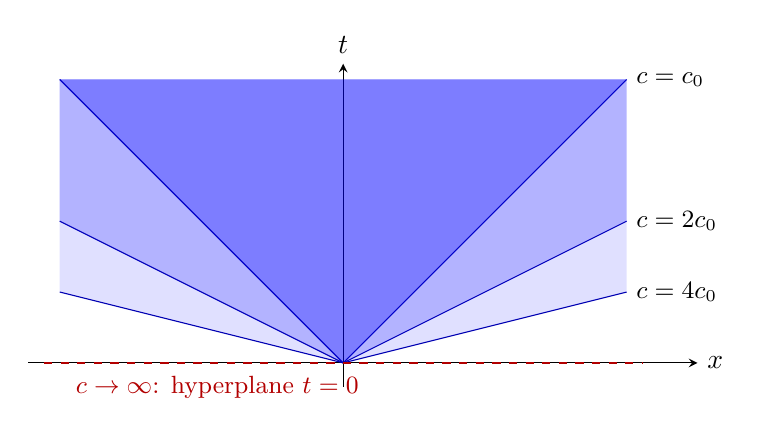
\begin{tikzpicture}[>=stealth]
\draw[->] (-4,0) -- (4.5,0) node[right] {$x$};
\draw[->] (0,-0.3) -- (0,3.8) node[above] {$t$};
\foreach \c/\op in {1/0.30, 2/0.20, 4/0.12}{
  \fill[blue,opacity=\op] (0,0) -- (-3.6,{3.6/\c}) -- (-3.6,3.6) -- (3.6,3.6) -- (3.6,{3.6/\c}) -- cycle;
  \draw[blue!70!black] (-3.6,{3.6/\c}) -- (0,0) -- (3.6,{3.6/\c});
}
\node[right,font=\small] at (3.6,3.6) {$c=c_0$};
\node[right,font=\small] at (3.6,1.8) {$c=2c_0$};
\node[right,font=\small] at (3.6,0.9) {$c=4c_0$};
\draw[red!70!black,dashed,thick] (-3.8,0) -- (3.8,0);
\node[below,font=\small,red!70!black] at (-1.6,-0.05) {$c\to\infty$: hyperplane $t=0$};
\end{tikzpicture}
\caption{The future cones $\{t>|x|/c\}$ for increasing $c$. The boundary flattens onto the
simultaneity hyperplane; the limit is a foliation, not a cone.}\label{fig:cones}
\end{figure}

\subsection{Connections and the non-uniqueness of inertial structure}
On a Lorentzian manifold the Levi-Civita connection is determined uniquely by the metric. On a
Galilean manifold the conditions $\nabla\tau=0$, $\nabla h^{-1}=0$, together with vanishing torsion,
do \emph{not} fix $\nabla$. If $\nabla$ and $\nabla'$ are two such connections, then
\begin{equation}
\Gamma'^{\lambda}{}_{\mu\nu}-\Gamma^{\lambda}{}_{\mu\nu}
=h^{\lambda\sigma}\bigl(\tau_\mu F_{\sigma\nu}+\tau_\nu F_{\sigma\mu}\bigr)
\end{equation}
for some two-form $F$ \cite{Kunzle72,DBKP85}. (One checks directly that this preserves $\nabla\tau=0$ and $\nabla h^{-1}=0$.)
This freedom contains Coriolis-type inertial forces and the gradient of a Newtonian gravitational
potential, which therefore appears as part of the connection and must be fixed by further
postulates. In general relativity the metric alone determines the connection, and gravity is the
dynamics of the metric. Consequently the Newtonian limit of general relativity is only well
defined once formulated in Newton--Cartan language, with rescaled data $(\tau,h^{-1},\nabla)$
\cite{Kunzle72,DBKP85,Ehlers97}; this is again a limit of structures that changes the type of
structure.

\subsection{One-particle phase space: where the limit is regular}
There is one place where the contraction is smooth. The mass shell of a massive particle in
Minkowski momentum space is the hyperboloid $p_\mu p^\mu=m^2c^2$, i.e.\ $p^0=\sqrt{|\bp|^2+m^2c^2}$ with $p^0=H/c$. For
signature $(+,-,-,-)$ the metric induced on it is negative definite; in the coordinates
$\bp\in\R^3$ the Riemannian metric obtained by reversing its sign is
\begin{equation}
\dd\ell^2=|\dd\bp|^2-\frac{(\bp\cdot\dd\bp)^2}{|\bp|^2+m^2c^2},
\end{equation}
a hyperbolic space $H^3$ of constant curvature $-1/(mc)^2$. As $c\to\infty$ the curvature tends to
zero and $\dd\ell^2\to|\dd\bp|^2$, the flat metric of $\R^3$, which is the momentum space on which
Galilean boosts act by translation $\bp\mapsto\bp+M\bu$. Thus the coadjoint orbit of the Poincar\'e
group describing a massive spinless particle converges, as a homogeneous Riemannian space
(pointed Gromov--Hausdorff sense), to the orbit of the Bargmann group \cite{Souriau70}. In the
language of Section~\ref{sec:limits}: the singularity of the contraction sits in the group and in
the spacetime, while the single-particle orbit contracts regularly. This explains why single-particle
phenomena tend to have non-relativistic limits, and we shall use this in Section~\ref{sec:EM}.

\begin{table}[ht]
\centering
\renewcommand{\arraystretch}{1.25}
\begin{tabular}{@{}>{\raggedright\arraybackslash}p{3.2cm}>{\raggedright\arraybackslash}p{5.6cm}>{\raggedright\arraybackslash}p{5.6cm}@{}}
\toprule
 & Minkowski & Galilei / Newton--Cartan \\
\midrule
Basic structure & Lorentzian metric $g_c=c^2\dd t^2-\dd\bx^2$ & absolute time $\tau=\dd t$, degenerate spatial metric $h^{-1}$ \\
Causal structure & light cones, finite speed $c$ & foliation by hyperplanes $t=\text{const}$ \\
Invariants of two events & $c^2\Delta t^2-|\Delta\bx|^2$ & $\Delta t$; $|\Delta\bx|$ if $\Delta t=0$ \\
Compatible connection & unique (Levi-Civita) & affine space over two-forms \\
Isometries of flat model & Poincar\'e group & Galilei group (Bargmann group on lifts) \\
Momentum space of mass $m$ & hyperboloid $H^3$, radius $mc$ & flat $\R^3$ (regular limit) \\
\bottomrule
\end{tabular}
\caption{Geometric structure.}\label{tab:geometry}
\end{table}

%=====================================================================
\section{Dynamics of interacting particles}\label{sec:dynamics}
%=====================================================================
Newtonian mechanics of $N$ particles with an interaction potential,
\begin{equation}
H=\sum_a\frac{\bp_a^2}{2m_a}+\sum_{a<b}V(|\bx_a-\bx_b|),\qquad
\bP=\sum_a\bp_a,\quad \mathbf K=\sum_a m_a\bx_a-t\bP,\quad \bJ=\sum_a\bx_a\times\bp_a,
\end{equation}
realises the Galilei algebra with canonical coordinates, for \emph{any} translation- and
rotation-invariant instantaneous potential: one checks $\{K_i,H\}=P_i$ because $V$ depends only on
differences of simultaneous positions. Galilean invariance imposes no restriction on the
interaction.

The relativistic analogue does not exist. The \emph{no-interaction theorem}
\cite{CJS63,Leutwyler65} states, informally, that if $N\ge2$ particles are described by a
Hamiltonian system on a phase space with canonical coordinates $(\bx_a,\bp_a)$, such that the ten
Poincar\'e generators are phase-space functions closing under the Poisson bracket and the $\bx_a$ are
world-line coordinates transforming as events under boosts, then the dynamics is free.
Relativistic interaction needs additional degrees of freedom (fields), or non-canonical
positions as in the Bakamjian--Thomas construction \cite{BT53}, or abandons manifest cluster
decomposition. There is therefore no family $T_c$ of Hamiltonian particle theories of the same
type with $T_\infty$ the Newtonian $N$-body problem. The relation is asymptotic: eliminating the
field, one obtains an expansion in $\kappa$ such as the Darwin Lagrangian \cite{Darwin20} (Gaussian
units, $a<b$ pairs, $\mathbf n_{ab}=(\bx_a-\bx_b)/r_{ab}$),
\begin{equation}
L=\sum_a\Bigl(\tfrac12m_av_a^2+\tfrac{1}{8c^2}m_av_a^4\Bigr)-\sum_{a<b}\frac{q_aq_b}{r_{ab}}
+\sum_{a<b}\frac{q_aq_b}{2c^2r_{ab}}\Bigl[\bv_a\!\cdot\!\bv_b+(\bv_a\!\cdot\!\mathbf n_{ab})(\bv_b\!\cdot\!\mathbf n_{ab})\Bigr]
+O(c^{-4}),
\end{equation}
which is Poincar\'e invariant only to the order retained, and which already ignores radiation. At the
level of Section~\ref{sec:limits}: reading (A) holds order by order for slow motion, but reading (B)
fails, since the structure at $\kappa=0$ (a closed canonical Hamiltonian theory with Galilean
symmetry) has no continuous counterpart for $\kappa>0$.

%=====================================================================
\section{A system that does have a limit: a charged particle in an external field}\label{sec:EM}
%=====================================================================

\subsection{Units: why Gaussian}\label{ssec:units}
In SI units the constants obey $\eps_0\mu_0c^2=1$. Consequently ``let $c\to\infty$'' is not a
well-defined instruction until one says which of $\eps_0$ and $\mu_0$ (equivalently, which unit of
charge) is held fixed, and the choice changes the limit. With $\eps_0$ fixed, $\mu_0=1/\eps_0c^2\to0$
and magnetic effects are suppressed. With $\mu_0$ fixed, $\eps_0\to0$, the Coulomb coupling
$q^2/4\pi\eps_0=\mu_0c^2q^2/4\pi$ grows like $c^2$ at fixed charge, and charges or charge densities
must be rescaled. An SI statement such as ``keep $\phi,\bA$ independent of $c$'' therefore conceals
an assumption about $\eps_0$.

In the Gaussian system the unit of charge is fixed by Coulomb's law, which contains no $c$, and $c$
enters only through explicit factors $1/c$ in the magnetic and induction terms. The content of
a $c\to\infty$ limit is then exactly the assignment of powers of $c$ to fields and sources, which is
what has to be specified. We use Gaussian units throughout this section, as already done for the
Darwin Lagrangian.

\subsection{Classical mechanics}\label{ssec:classical}
Take $x^0=ct$, signature $(+,-,-,-)$ and $A^\mu=(\phi,\bA)$. Maxwell's equations are
\begin{equation}\label{eq:maxwell}
\nabla\!\cdot\!\bE=4\pi\rho,\quad
\nabla\!\times\!\bB-\frac1c\,\partial_t\bE=\frac{4\pi}{c}\,\bJ,\quad
\nabla\!\times\!\bE+\frac1c\,\partial_t\bB=0,\quad
\nabla\!\cdot\!\bB=0,
\end{equation}
with $\bE=-\nabla\phi-\frac1c\partial_t\bA$, $\bB=\nabla\times\bA$ and
$\partial_t\rho+\nabla\!\cdot\!\bJ=0$. A particle of mass $m$ and charge $q$ feels the force
$q(\bE+\frac{\bv}{c}\times\bB)$; its action $S=-mc\int\dd s-\frac qc\int A_\mu\,\dd x^\mu$ gives
\begin{equation}\label{eq:Lc}
L_c=-mc^2\sqrt{1-v^2/c^2}+\frac qc\,\bv\cdot\bA-q\phi .
\end{equation}
Magnetism is, in this setting, a relativistic effect. The field of a single carrier of charge $q$ and
velocity $\bv$ is $B\sim qv/(cr^2)=O(1/c)$, and the current--current term of the Darwin Lagrangian
is $O(c^{-2})$. For a fixed finite number of particles the magnetic interaction therefore
disappears as $c\to\infty$ (this is the electric limit of Section~\ref{ssec:Galileanlimits}).
A \emph{finite} non-relativistic magnetic force $q\bv\times\tilde\bB$ arises only from macroscopic
sources, namely currents in neutral conductors or magnetisation, i.e.\ from a \emph{double limit}
$c\to\infty$, $N\to\infty$. Each carrier contributes $O(1/c)$ to $\bB$, and so does each elementary
magnetic moment $q\hbar/2mc$, so one needs $N\sim c^2$ carriers of fixed charge, with a
neutralising background so that the net $\bE$ stays $O(1)$. In terms of fields this means $\bB=O(c)$
when $\bE=O(1)$. We therefore put
\begin{equation}\label{eq:magscaling}
\bA=c\,\tilde\bA,\qquad \bB=c\,\tilde\bB,\quad\tilde\bB=\nabla\times\tilde\bA,\qquad
\bE=-\nabla\phi-\partial_t\tilde\bA,
\end{equation}
and take $(\phi,\tilde\bA)$ independent of $c$. This is the \emph{magnetic scaling} of
Section~\ref{ssec:Galileanlimits}: it is the form imposed by a macroscopic source prepared in the
double limit above, and the only one that keeps the Lorentz force. The ``prescribed external field''
is thus an idealisation of a macroscopic neutral source ($N\sim c^2$ carriers) whose own dynamics
is neglected. Then
\begin{equation}
L_c=-mc^2+\tfrac12mv^2+\frac{mv^4}{8c^2}+q\,\bv\cdot\tilde\bA-q\phi+O(c^{-4}).
\end{equation}
The constant $-mc^2=\frac{\dd}{\dd t}(-mc^2t)$ is a total derivative and does not affect the
Euler--Lagrange equations, even though it diverges. The equation of motion
$\frac{\dd}{\dd t}(\gamma m\bv)=q(\bE+\bv\times\tilde\bB)$ can be solved for the acceleration using
$m\,\dd\gamma/\dd t=q\,\bE\cdot\bv/c^2$ (the magnetic force does no work):
\begin{equation}
\dot{\bv}=\frac{q}{\gamma m}\Bigl[\bE+\bv\times\tilde\bB-\frac{\bv(\bv\cdot\bE)}{c^2}\Bigr],
\qquad\gamma=(1-\kappa v^2)^{-1/2}.
\end{equation}
The right-hand side is real-analytic in $\kappa$ near $\kappa=0$ for fixed $(\bx,\bv,t)$ with
$|\bv|<c$. Hence this is a \emph{regular} perturbation problem.

\begin{proposition}
Let $\phi,\tilde\bA$ be smooth and $c$-independent, and let $(\bx_0,\bv_0)$ be fixed initial data.
Let $\bx_0(t)$ solve the Newton--Lorentz equation $m\ddot\bx=q(\bE+\dot\bx\times\tilde\bB)$ on
$[0,T]$. For $\kappa$ small enough the relativistic solution $\bx_\kappa(t)$ with the same initial
data exists on $[0,T]$ and $\bx_\kappa=\bx_0+O(\kappa)$ in $C^k([0,T])$ for every~$k$.
\end{proposition}
\begin{proof}
Continuous (indeed analytic) dependence of solutions of ODEs on parameters. The solution $\bx_0$
is bounded in velocity on $[0,T]$, so $|\bv|<c$ along it for large $c$, and a neighbouring
solution stays in the domain of analyticity. \qedhere
\end{proof}

The \emph{symmetry} structure also passes to the limit. Under a Lorentz boost with velocity $\bu$ the
four-potential transforms as $\phi'=\gamma(\phi-\frac{\bu}{c}\cdot\bA_\parallel)$,
$\bA'_\parallel=\gamma(\bA_\parallel-\frac{\bu}{c}\phi)$, $\bA'_\perp=\bA_\perp$. In terms of
$(\phi,\tilde\bA)$, with $\bA=c\tilde\bA$, this becomes in the limit $c\to\infty$
\begin{equation}\label{eq:magtransf}
\tilde\bA'(\bx',t)=\tilde\bA(\bx,t),\qquad
\phi'(\bx',t)=\phi(\bx,t)-\bu\cdot\tilde\bA(\bx,t),\qquad
\bx'=\bx-\bu t,
\end{equation}
so that $\bE'=\bE+\bu\times\tilde\bB$ and $\tilde\bB'=\tilde\bB$. Then
$L_N=\tfrac12mv^2+q\bv\cdot\tilde\bA-q\phi$ satisfies
\begin{equation}
L_N'=L_N-\frac{\dd}{\dd t}\Bigl(m\,\bu\cdot\bx-\tfrac12mu^2t\Bigr),
\end{equation}
i.e.\ it is invariant up to a total derivative whose generating function is the mass cocycle of
Section~\ref{ssec:mass}. The group, the cocycle and the coupling are all consistent in the limit.

\subsection{Two Galilean limits of electromagnetism}\label{ssec:Galileanlimits}
The scaling \eqref{eq:magscaling} is not the only possible one. Le Bellac and L\'evy-Leblond
\cite{LBLL73} (see also \cite{Rousseaux13}) showed that Maxwell theory has \emph{two}
inequivalent Galilean-covariant limits. In Gaussian units they correspond to two ways of assigning
powers of $c$ to $\bE,\bB,\rho,\bJ$ in \eqref{eq:maxwell}; the regimes are $|\bE|\gg|\bB|$ and
$|\bE|\ll|\bB|$, and the sources must scale accordingly (Table~\ref{tab:galileanEM}).

\begin{table}[ht]
\centering
\renewcommand{\arraystretch}{1.25}
\begin{tabular}{@{}>{\raggedright\arraybackslash}p{2.3cm}>{\raggedright\arraybackslash}p{6.0cm}>{\raggedright\arraybackslash}p{6.0cm}@{}}
\toprule
 & Electric limit & Magnetic limit \\
\midrule
Scaling as $c\to\infty$ & $\bE,\rho,\bJ,\phi=O(1)$; $\ \bB=\bB_1/c$, $\bA=\bA_1/c$ & $\bE,\rho,\phi=O(1)$; $\ \bB=c\tilde\bB$, $\bA=c\tilde\bA$, $\bJ=c^2\tilde\bJ$ \\
Regime & $|\bE|\gg|\bB|$, $|\bJ|\ll c|\rho|$ & $|\bE|\ll|\bB|$, $|\bJ|\gg c|\rho|$ \\
Boost law & $\bE'=\bE$, $\ \bB_1'=\bB_1-\bu\times\bE$ & $\bE'=\bE+\bu\times\tilde\bB$, $\ \tilde\bB'=\tilde\bB$ \\
Field equations & $\nabla\!\cdot\!\bE=4\pi\rho$, $\nabla\!\times\!\bE=0$, $\nabla\!\cdot\!\bB_1=0$, $\nabla\!\times\!\bB_1-\partial_t\bE=4\pi\bJ$ & $\nabla\!\cdot\!\bE=4\pi\rho$, $\nabla\!\times\!\bE+\partial_t\tilde\bB=0$, $\nabla\!\cdot\!\tilde\bB=0$, $\nabla\!\times\!\tilde\bB=4\pi\tilde\bJ$ \\
Force on a test charge & $q\bE$ (magnetic force is $O(c^{-2})$) & $q(\bE+\bv\times\tilde\bB)$ \\
Particle Lagrangian & $\tfrac12mv^2-q\phi$ & $\tfrac12mv^2+q\bv\cdot\tilde\bA-q\phi$ \\
Character & electroquasistatics; displacement current kept, induction dropped & magnetoquasistatics; induction kept, displacement current dropped \\
\bottomrule
\end{tabular}
\caption{The two Galilean limits of electromagnetism in Gaussian units: scalings of fields and sources, field sector, and induced test-particle dynamics.}\label{tab:galileanEM}
\end{table}

One checks directly that inserting the scalings in \eqref{eq:maxwell} leaves the displayed equations
at leading order. In the electric limit $\bB=O(1/c)$ enters the induction law only at order $c^{-2}$,
which gives $\nabla\times\bE=0$, while the displacement current and $\bJ$ enter Amp\`ere's law at the
same order as $\nabla\times\bB_1$. In the magnetic limit $\bJ=c^2\tilde\bJ$ is needed to balance
$c\,\nabla\times\tilde\bB$; the displacement current is then $O(c^{-2})$ and drops out, and
continuity reduces to $\nabla\!\cdot\!\tilde\bJ=0$. The factor $c^2$ in $\bJ$ is the double limit $c\to\infty$, $N\to\infty$ of
Section~\ref{ssec:classical}: the force between two current elements is of relative order
$v^2/c^2$ compared with the Coulomb forces between the individual charge carriers, so a
quasi-neutral conductor must carry opposite charge densities of order $c^2$ ($N\sim c^2$ carriers
of fixed charge) whose sum is $O(1)$. The two limits thus differ in kind. The electric limit is a
limit at fixed sources, i.e.\ of a fixed few-body theory. The magnetic limit is a collective limit of
a macroscopic neutral source, and it is not a limit of any fixed system. Neither scaling is
``Maxwell's equations with $c$ dropped'', and the two are inequivalent.

Holding $(\phi,\tilde\bA)$ fixed selects the magnetic limit, which is why \eqref{eq:Lc} yields the
full Newton--Lorentz equation. In the electric scaling $\bA=\bA_1/c$ the term
$\frac qc\bv\cdot\bA$ in \eqref{eq:Lc} is $O(c^{-2})$ and the particle feels only $q\bE$. The field
sector in both limits is \emph{instantaneous}: no wave equation survives (the electric limit is
Coulombic, the magnetic one diffusive). Radiation, retardation and a finite signal speed are
not recovered; they are precisely what is destroyed by the contraction of the spacetime structure
of Section~\ref{sec:geometry}. The limit of the \emph{particle} sector therefore does not extend to
the \emph{field} sector as a limit of the same type of theory.

\subsection{Quantum mechanics}
Write $\boldsymbol\pi=\mathbf p-\frac qc\bA=\mathbf p-q\tilde\bA$ with $\mathbf p=-\ii\hbar\nabla$; in the
magnetic scaling $\boldsymbol\pi$ is independent of $c$. For the Klein--Gordon equation in the field,
$(\ii\hbar\partial_t-q\phi)^2\psi=c^2\boldsymbol\pi^2\psi+m^2c^4\psi$, the limit $c\to\infty$ at fixed
$\psi$ does not exist: the equation is second order in time and $\psi$ oscillates like
$e^{\mp\ii mc^2t/\hbar}$. The remedy is to remove the rapidly oscillating phase,
$\psi=e^{-\ii mc^2t/\hbar}\varphi$, which yields (exactly)
\begin{equation}\label{eq:KG}
\ii\hbar\,\partial_t\varphi=\Bigl[\frac{\boldsymbol\pi^2}{2m}+q\phi\Bigr]\varphi-\frac{1}{2mc^2}\bigl(\ii\hbar\partial_t-q\phi\bigr)^2\varphi .
\end{equation}
The last term is $O(\kappa)$ on slowly varying positive-energy states and is dropped in the limit,
which is the Schr\"odinger equation. The small parameter multiplies the highest time derivative:
this is a singular perturbation, which changes the order of the equation from two to one and
removes the negative-frequency branch ($e^{+\ii mc^2t/\hbar}\chi$). The phase factor is the quantum
manifestation of the central term \eqref{eq:shift}, i.e.\ of the Bargmann cocycle.

For spin $\tfrac12$, the Dirac Hamiltonian $H_D=c\,\boldsymbol\alpha\cdot\boldsymbol\pi+\beta mc^2+q\phi$ is block-diagonalised, order by order in $1/mc^2$, by the
Foldy--Wouthuysen transformation \cite{FW50}. Using
$(\boldsymbol\sigma\cdot\boldsymbol\pi)^2=\boldsymbol\pi^2-\frac{\hbar q}{c}\,\boldsymbol\sigma\cdot\bB$, the leading upper-block equation (after subtracting $mc^2$) is the Pauli equation
\begin{equation}\label{eq:Pauli}
\ii\hbar\,\partial_t\chi=\Bigl[\frac{(\boldsymbol\sigma\cdot\boldsymbol\pi)^2}{2m}+q\phi\Bigr]\chi
=\Bigl[\frac{(\mathbf p-\frac qc\bA)^2}{2m}-\frac{q\hbar}{2mc}\,\boldsymbol\sigma\cdot\bB+q\phi\Bigr]\chi ,
\end{equation}
with gyromagnetic ratio $g=2$. In the magnetic scaling \eqref{eq:magscaling} all factors of $c$ in
\eqref{eq:Pauli} disappear, $\frac qc\bA=q\tilde\bA$ and $\frac qc\bB=q\tilde\bB$, which is why this
scaling has a finite limit; in the electric scaling $\boldsymbol\pi\to\mathbf p$ and the Pauli term
vanishes. Higher orders in $\kappa$ give the relativistic kinetic correction, the spin--orbit
coupling and the Darwin term. L\'evy-Leblond \cite{LL67} showed that a first-order,
Galilei-invariant spinor equation, obtained as a contraction of the Dirac equation and not
referring to $c$, yields the Pauli equation directly: here the limit exists at the level of the
wave equation and its symmetry group together.

\subsection{Why this system has a limit}\label{ssec:why}
The structural features of the previous sections explain the success of the limit for a test
particle and, by the same token, its limits of validity.
\begin{enumerate}[label=(\roman*),itemsep=2pt]
\item \emph{The one-particle orbit contracts regularly.} The mass-shell hyperboloid has curvature
$-1/(mc)^2\to0$ (Section~\ref{sec:geometry}); the particle's kinematics converges to that of
the Bargmann group.
\item \emph{The divergence is central and removable.} The only divergent quantity is the rest
energy $mc^2$, a central term. Subtracting it \eqref{eq:shift} (classically, a total derivative;
quantum mechanically, a phase) turns the singular change of basis into a regular family.
\item \emph{The external field has no dynamics of its own, and an admissible scaling exists.} The
coupling is one-sided, and the potentials can be given an explicit scaling with $c$ (the magnetic
one, $\bA=c\tilde\bA$ in Gaussian units, which describes a macroscopic neutral source with
$N\sim c^2$ carriers) under which they transform as a representation of the
Galilei group \eqref{eq:magtransf}. The no-interaction theorem of Section~\ref{sec:dynamics} does
not apply, since the field is not a degree of freedom of a particle Hamiltonian system and
explicitly breaks translation invariance anyway.
\item \emph{Pair creation is suppressed.} The one-particle description requires the field to be
well below the Schwinger critical value $E_S=m^2c^3/(|q|\hbar)$ \cite{Schwinger51}, which tends
to infinity as $c\to\infty$ for fields with $\bE=O(1)$.
\end{enumerate}
By contrast, as soon as the field becomes dynamical (radiation reaction, retardation, the
many-body problem of Section~\ref{sec:dynamics}), one or more of these conditions fails. We offer
(i)--(iv) as a heuristic criterion, not as a theorem: \emph{a subsystem has a non-relativistic
limit when its phase space contracts regularly, its divergent terms are central, and all its
couplings can be assigned powers of $c$ so as to carry a representation of the contracted group
(for magnetic couplings this includes a simultaneous large-$N$ limit of the sources).}

%=====================================================================
\section{Conclusions}\label{sec:conclusion}
%=====================================================================
\begin{itemize}[itemsep=2pt]
\item The relation between Newtonian and relativistic mechanics is a contraction, not a regular
limit: the Galilei algebra is the singular limit of a family of Poincar\'e algebras related by
rescalings that do not converge, and it is not isomorphic to them (different Levi factor and
radical, non-trivial central extension, no four-vector structure, no invariant quadratic form on
energy--momentum).
\item The geometry changes in kind: a Lorentzian metric is replaced by a pair of degenerate
structures that do not determine the connection; the light cone collapses onto a foliation by
simultaneity hyperplanes.
\item The dynamics of interacting particles is Galilei-invariant for any instantaneous potential,
whereas Hamiltonian particle theories with canonical coordinates cannot be Poincar\'e-invariant
and interacting; the relation between them is an asymptotic series, not a limit of theories of the same type.
\item Nonetheless, individual systems can have non-relativistic limits. For a charged particle in a
prescribed electromagnetic field the limit holds classically (regular ODE perturbation, Lorentz
force, quasi-invariance with the mass cocycle) and quantum mechanically (Dirac $\to$ Pauli),
because the single-particle orbit contracts regularly, the divergence is a removable central term,
and the field can be given a scaling with $c$ under which it is Galilean-covariant. For the magnetic
part this is the scaling of a double limit $c\to\infty$, $N\to\infty$: for a fixed number of charges
magnetism is a relativistic effect, and it survives only for macroscopic currents or magnetisation.
The powers of $c$ are visible in Gaussian units and concealed in SI, where $\eps_0\mu_0c^2=1$
forbids holding both constants fixed. Electromagnetism itself has two
inequivalent Galilean limits (electric and magnetic), neither of which contains radiation.
\end{itemize}
The summary is that ``limit'' should always be accompanied by the specification of
\emph{what} converges: formulas and solutions of a given system, which often do; or the algebraic and
geometric structures of the theory, which do not.

%=====================================================================
\begin{thebibliography}{99}\small
\bibitem{Wigner39} E.~P. Wigner, On unitary representations of the inhomogeneous Lorentz group, \emph{Ann. Math.} \textbf{40} (1939) 149--204.
\bibitem{Segal51} I.~E. Segal, A class of operator algebras which are determined by groups, \emph{Duke Math. J.} \textbf{18} (1951) 221--265.
\bibitem{IW53} E. In\"on\"u and E.~P. Wigner, On the contraction of groups and their representations, \emph{Proc. Natl. Acad. Sci. USA} \textbf{39} (1953) 510--524.
\bibitem{Bargmann54} V. Bargmann, On unitary ray representations of continuous groups, \emph{Ann. Math.} \textbf{59} (1954) 1--46.
\bibitem{Saletan61} E.~J. Saletan, Contraction of Lie groups, \emph{J. Math. Phys.} \textbf{2} (1961) 1--21.
\bibitem{LL63} J.-M. L\'evy-Leblond, Galilei group and nonrelativistic quantum mechanics, \emph{J. Math. Phys.} \textbf{4} (1963) 776--788.
\bibitem{LL67} J.-M. L\'evy-Leblond, Nonrelativistic particles and wave equations, \emph{Commun. Math. Phys.} \textbf{6} (1967) 286--311.
\bibitem{BLL68} H. Bacry and J.-M. L\'evy-Leblond, Possible kinematics, \emph{J. Math. Phys.} \textbf{9} (1968) 1605--1614.
\bibitem{LBLL73} M. Le Bellac and J.-M. L\'evy-Leblond, Galilean electromagnetism, \emph{Nuovo Cimento B} \textbf{14} (1973) 217--233.
\bibitem{Rousseaux13} G. Rousseaux, Forty years of Galilean electromagnetism (1973--2013), \emph{Eur. Phys. J. Plus} \textbf{128} (2013) 81.
\bibitem{Cartan23} \'E. Cartan, Sur les vari\'et\'es \`a connexion affine et la th\'eorie de la relativit\'e g\'en\'eralis\'ee (premi\`ere partie), \emph{Ann. Sci. \'Ecole Norm. Sup.} \textbf{40} (1923) 325--412.
\bibitem{Kunzle72} H.~P. K\"unzle, Galilei and Lorentz structures on space-time: comparison of the corresponding geometry and physics, \emph{Ann. Inst. H. Poincar\'e A} \textbf{17} (1972) 337--362.
\bibitem{DBKP85} C. Duval, G. Burdet, H.~P. K\"unzle and M. Perrin, Bargmann structures and Newton--Cartan theory, \emph{Phys. Rev. D} \textbf{31} (1985) 1841--1853.
\bibitem{Ehlers97} J. Ehlers, Examples of Newtonian limits of relativistic spacetimes, \emph{Class. Quantum Grav.} \textbf{14} (1997) A119--A126.
\bibitem{Souriau70} J.-M. Souriau, \emph{Structure des syst\`emes dynamiques}, Dunod, Paris, 1970.
\bibitem{CJS63} D.~G. Currie, T.~F. Jordan and E.~C.~G. Sudarshan, Relativistic invariance and Hamiltonian theories of interacting particles, \emph{Rev. Mod. Phys.} \textbf{35} (1963) 350--375.
\bibitem{Leutwyler65} H. Leutwyler, A no-interaction theorem in classical relativistic Hamiltonian particle dynamics, \emph{Nuovo Cimento} \textbf{37} (1965) 556--567.
\bibitem{BT53} B. Bakamjian and L.~H. Thomas, Relativistic particle dynamics. II, \emph{Phys. Rev.} \textbf{92} (1953) 1300--1310.
\bibitem{Darwin20} C.~G. Darwin, The dynamical motions of charged particles, \emph{Phil. Mag.} \textbf{39} (1920) 537--551.
\bibitem{FW50} L.~L. Foldy and S.~A. Wouthuysen, On the Dirac theory of spin 1/2 particles and its non-relativistic limit, \emph{Phys. Rev.} \textbf{78} (1950) 29--36.
\bibitem{Schwinger51} J. Schwinger, On gauge invariance and vacuum polarization, \emph{Phys. Rev.} \textbf{82} (1951) 664--679.
\bibitem{Nickles73} T. Nickles, Two concepts of intertheoretic reduction, \emph{J. Philosophy} \textbf{70} (1973) 181--201.
\bibitem{Dyson72} F.~J. Dyson, Missed opportunities, \emph{Bull. Amer. Math. Soc.} \textbf{78} (1972) 635--652.
\bibitem{VM94} R. Vilela Mendes, Deformations, stable theories and fundamental constants, \emph{J. Phys. A} \textbf{27} (1994) 8091--8104.
\bibitem{Berry94} M.~V. Berry, Asymptotics, singularities and the reduction of theories, in \emph{Logic, Methodology and Philosophy of Science IX}, Elsevier, 1994, pp.~597--607.
\bibitem{Batterman02} R.~W. Batterman, \emph{The Devil in the Details}, Oxford University Press, 2002.
\end{thebibliography}

\end{document}
